\documentclass[12pt,a4paper,utf8]{ctexart}
\usepackage{ctex,amsmath,amssymb,subfig,diagbox,cite,graphicx,fontspec}
\usepackage[ntheorem]{empheq}
\usepackage{enumitem,fullpage,cleveref,cellspace,listings,color,framed}
\definecolor{gray}{rgb}{0.5,0.5,0.5}
\definecolor{dkgreen}{rgb}{.068,.578,.068}
\definecolor{dkpurple}{rgb}{.320,.064,.680}

%set fortran styles
\lstset{
    frameround=tftf,
    language=Fortran,
    keywords={SELECT,PROGRAM,PRINT,STOP,END,WRITE,INTEGER,REAL,COMPLEX,CHARACTER,LOGICAL,READ,FORMAT,IMPLICIT,PARAMETER,DATA,EQUIVALENCE,TYPE,PAUSE,CONTINUE,CYCLE,EXIT,IF,SELECT,DO,ALLOCATE,DEALLOCATE,WHERE,FORALL,SUBROUTIHNE,CALL,RETURN,FUNCTION,COMMON,BLOCK DATA,SAVE,INTERFACE,CONTAIN,MODULE,USE,PUBLIC,PRIVATE,ENTRY,OPEN,INQUIRE,CLOSE,NAMELIST,POINTER,NULLFY,REWIND,BACKSPACE,ENDFILE
    },
    basicstyle=\small\ttfamily,
    numbers=left,
    numberstyle=\small,
    keywordstyle=\color{blue}\bfseries,
    commentstyle=\color{dkgreen},
    stringstyle=\color{dkpurple},
    backgroundcolor=\color{white},
    tabsize=2,
    showspaces=false,
    showstringspaces=false,
    breaklines=true,
    frame=trBL
}
\CTEXsetup[format+={\raggedright}]{section}
\begin{document}
\begin{center}
    {\LARGE\textbf{计算物理 作业一}}\\
    \textrm{于浩然}~~~~~~\textrm{PB19020634}~~~~~~\textrm{2021.10.04}
\end{center}
\section{作业题目}
用Schrage方法编写随机数子程序,用指定间隔(非连续$l>1$)两个随机数作为点的坐标值绘出若干点的平面分布图。再用$\langle
x^k
\rangle$测试均匀性(取不同量级的$N$值,讨论偏差与$N$的关系)、$C(l)$测试其二维独立性(总点数$N>10^7$)。
\section{算法简介}
\begin{enumerate}
    \item[(a)] \textbf{Schrage方法简介}\\
最简单的均匀随机数产生器是线性同余法产生器
\textsl{(LCG)},随机数序列${x_n}$按线性关系得到,其原理如下:\\
\begin{eqnarray}
    I_{n+1}&=&(aI_n+b)\mathrm{mod} m \\
    x_n&=&I_n/m
\end{eqnarray}
具体举例,有一种通过了许多理论测试和实用性考验的LCG,它通常被叫做"16807"产生器,其参数满足:
\begin{equation}
    a=7^5=16807,\quad b=0,\quad m=2^{31}-1=2147483647
\end{equation}
但在具体运算中,$aI_n$很可能在取模前就超过计算机能够表示的最大整数值,故需要设计一种让计算机能够在其运算范围内取模的方法,亦即我们所采用的Schrage方法:\\
设$m$可表为
\begin{equation}
    m=aq+r,\quad q=[m/a],\quad r= m\mathrm{mod} a
\end{equation}
则$aI_n\mathrm{mod}m$可用如下等式表达
\begin{equation}
    aI_n\mathrm{mod} m=\left\{
    \begin{aligned}
        I_n(z\mathrm{mod} q)-r[z/q]\qquad &,if\geqslant 0 \\
        I_n(z\mathrm{mod} q)-r[z/q]+m &,otherwise
    \end{aligned}
    \right.
\end{equation}
    \item[(b)] \textbf{k阶矩检验均匀性}\\
        均匀性是指在 $[0,1]$区间内等长度子区间中随机数的数量相同。
        对于均匀分布的随机变量$x$,其 $k$阶矩满足如下关系:
\begin{equation}
    \langle x^k \rangle= \frac{1}{N} \sum_{i=1}^{N}x_i^k \Rightarrow \int_0^1
    x^k p(x) \textrm{d}x = \frac{1}{k+1}
\end{equation}
上面(6)式中 $p(x)$为均匀分布的概率密度函数,其值为 $1$.\\
\begin{equation}
    \left | \langle x^k \rangle - \frac{1}{k+1} \right | \approx\mathcal{O} \left (
    \frac{1}{\sqrt{N}} \right )
\end{equation}
由上述关系,可通过计算随机数的 $k$阶矩来检验其均匀性, $\left | \langle x^k
\rangle - \frac{1}{k+1} \right | $越小说明其均匀性越好。
    \item[(c)] \textbf{自相关系数检验2维独立性}\\
        独立性是指按先后顺序出现的随 机数中,每个随机数的取值与其相距一定间隔的随机数取值之间无关。我们使用的讨论随机数序列独立性的方法是顺序相关法,它用相距一定距离的两个随机数的自相关函数(或相关系数)来标识伪随机数序列的独立性情况,表达式如下:
\begin{equation}
    C(l)= \frac{\langle x_n x_{n+l} \rangle - \langle x_n \rangle ^2}{\langle
    x_n^2 \rangle - \langle x_n \rangle ^2}
\end{equation}
其中 $\langle x_n \rangle$ 表示平均值 $ \sum_{n+1}^{N}x_n /N$.相关系数小只能保证
$x_n$与 $x_{n+l}$之间线性关系弱,但无法保证不存在其他类型的函数关系。
\begin{equation}
    \left | C(l) \right | \approx \mathcal{O} \left ( \frac{1}{\sqrt{N}} \right
        )
\end{equation}
通过上述关系,我们可计算 $C(l)$的值来考察随机数的独立性。
\end{enumerate}
\section{编程实现}
采用最简单的16807生成器进行编程实现,由(3)(4)可得
\begin{equation}
    a=16807,\quad q=127773,\quad r=2836,\quad m=2147483647
\end{equation}
使用Fortran90进行编程,共包含三个子程序,功能简介与源代码如下:
\begin{itemize}
    \item \texttt{SUBROUTINE Schrage(P)}\\
        通过传入的参数
        \texttt{P}确定要生成的随机数数目
        $(10^P)$,为简单可重复起见我们采用的种子为
        \texttt{In(1) = m - 1}.按Schrage方法生成随机数并其存入实型数组
        \texttt{z},最后将数组 \texttt{z}写入文件 \texttt{rand.out}.
\begin{framed}
\begin{lstlisting}
SUBROUTINE Schrage(P) !Schrage随机数生成器子程序
   IMPLICIT NONE
   INTEGER :: N = 1, P 
   INTEGER :: m = 2147483647, a = 16807, q = 127773, r = 2836, In(10**P)
   REAL(KIND=8) z(10**P)
   In(1) = m - 1
   z(1) = REAL(In(1))/m
   DO N = 1, 10**P - 1
      In(N + 1) = a*MOD(In(N), q) - r*INT(In(N)/q)
      IF (In(N + 1) < 0) THEN !若值小于零,按Schrage方法加m
         In(N + 1) = In(N + 1) + m
      END IF
      z(N + 1) = REAL(In(N + 1))/m !得到第N+1个随机数
   END DO
   OPEN (1, file='rand.out') !每次运行子程序将覆盖随机数
   DO N = 1, 10**P !将随机数按行存入文件
      WRITE (1, *) z(N)
   END DO
   CLOSE (1)
END SUBROUTINE Schrage
\end{lstlisting}
\end{framed}
    \item \texttt{SUBROUTINE Moment(P)}\\
        由传入参数 \texttt{P}确定随机数组大小,读取先前生成的包含
        $10^P$个随机数的文件
        \texttt{rand.out}写入实型数组 \texttt{z},根据(6)计算出 $k$阶矩的值
        \texttt{S(k)},由(7)计算出 $k$阶矩的偏差 \texttt{D(k)},分别写入文件
        \texttt{monments.out}和 \texttt{difference.out}.
\begin{framed}
\begin{lstlisting}
SUBROUTINE Moment(P) !k阶矩均匀性检验子程序(N一定)
    INTEGER(KIND=4) :: i = 1, k = 1, P
    REAL(KIND=8), DIMENSION(10) :: S = 0, D = 0
    REAL(KIND=8) :: z(10**P)
    OPEN (1,file='rand.out') !从前面产生的'rand.out'文件中读取随机数表
    READ (1, *) z
    CLOSE (1)
    DO k = 1, 10 !求随机数的1阶矩至10阶矩
        S(k) = SUM(z**k) / SIZE(z)
        D(k) = ABS(S(k) - real(1) / (1 + k)) !求出各k值对应的偏差
    END DO
    OPEN (99, ACCESS='append', file='moments.out') !将k阶矩均值存入文件
    WRITE (99, *) S
    CLOSE(99)
    OPEN (3, ACCESS='append', file='difference.out') !将偏差存入文件
    WRITE (3, *) D
    CLOSE(3)
END SUBROUTINE Moment
\end{lstlisting}
\end{framed}
    \item \texttt{SUBROUTINE Independence(P)}\\
        由传入参数 \texttt{P}
        确定随机数组大小,读取文件写入实型数组(同上).根据公式(8)(9)计算
        $C(l)$,将结果写入文件 \texttt{indep.out}.
\begin{framed}
\begin{lstlisting}
SUBROUTINE Independence(P) !2维独立性检验子程序
    INTEGER(KIND=4) :: P, l = 1, i = 1
    REAL(KIND=8) :: ave = 0, coave = 0, sqrave = 0 !分别表示<x>,<x_i*x_{i+l}>,<x^2>
    REAL(KIND=8), DIMENSION(1:4) :: C
    REAL(KIND=8), DIMENSION(1:10**P) :: z
    OPEN (1, file='rand.out')
    READ (1, *) z
    CLOSE(1)
    ave = SUM(z) / SIZE(z) !求均值
    sqrave = SUM(z**2) / SIZE(z)
    DO l = 1, 4
        DO i = 1, 10**P - l
            coave = coave + z(i) * z(i + l)
        END DO
        DO i = 1, l !在这里将越界的z(i+l)替换为z(N+i-l)
            coave = coave + z(i) * z(10**P + i - l)
        END DO
        coave = coave / SIZE(z)
        C(l) = ABS((coave - ave**2)/(sqrave - ave**2)) !相关系数公式
    END DO
    OPEN (99, ACCESS='append', file='indep.out')
    WRITE (99, *) C !将相关系数值存入文件
    CLOSE (99)
END SUBROUTINE Independence
\end{lstlisting}
\end{framed}
\end{itemize}
在主程序中只需声明一个变量 \texttt{P},使用一个
\texttt{DO}循环结构,在随机数序列大小为 $10^2$ 到 $10^7$的各次幂时,分别调用上述子程序.
\begin{framed}
\begin{lstlisting}
PROGRAM MAIN
    IMPLICIT NONE
    INTEGER :: P=1 
    !PRINT *, 'How many random numbers are required?(10^P)'
    !READ *, P !从键盘读取随机数数量大小
    DO P = 2, 7
        CALL Schrage(P)
        CALL Moment(P)
        CALL Independence(P)
    END DO
END PROGRAM MAIN    
\end{lstlisting}
\end{framed}
为实现绘制散点图功能,使用了Python脚本,通过\texttt{matplotlib.pyplot.scatter}实现,源代码展示如下:
\begin{framed}
\begin{lstlisting}[language=python]
import matplotlib.pyplot as plt
import numpy as np
import matplotlib as mpl
plt.rcParams['savefig.dpi'] = 600
plt.rcParams['figure.dpi'] = 600

fig, ax = plt.subplots()
ax.set_aspect(1)
data = np.loadtxt("rand6.out")
LENGTH = 4000  # 绘制4000个点的散点图
#LENGTH = 20000 # 绘制20000个点的散点图
#LENGTH = 40000
x = np.zeros(LENGTH)
y = np.zeros(LENGTH)
for num in range(1, LENGTH):
    x[num] = data[num]
    y[num] = data[num + 3]  # 取l值为3  
plt.scatter(x, y, s=2)
ax.set_xlabel('x')
ax.set_ylabel('y')
plt.savefig("rand.png")
\end{lstlisting}
\end{framed}
\newpage
\section{计算结果}
\begin{enumerate}
    \item[(a)] \textbf{随机数平面分布图}\\
        运行Python脚本可得到给定种子一定数目随机数的平面分布图。种子一定时,生成不同数目随机数的前
        $N$个数都是相同的,故为了读取数据速度快直接读取 $10^6$个随机数的文件
        \texttt{rand6.out}.取l值为3,即 \texttt{y}坐标的随机数为对应
        \texttt{x}坐标的随机数后面的第三个数.取
        \texttt{LENGTH}分别为4000,20000,40000绘图,展示如下.可看出,16807产生的随机数具有很好的性质,在平面图上无法看出随机数间的关联性。
\begin{figure}[h]
    \centering
    \subfloat[4000个随机数平面分布图]{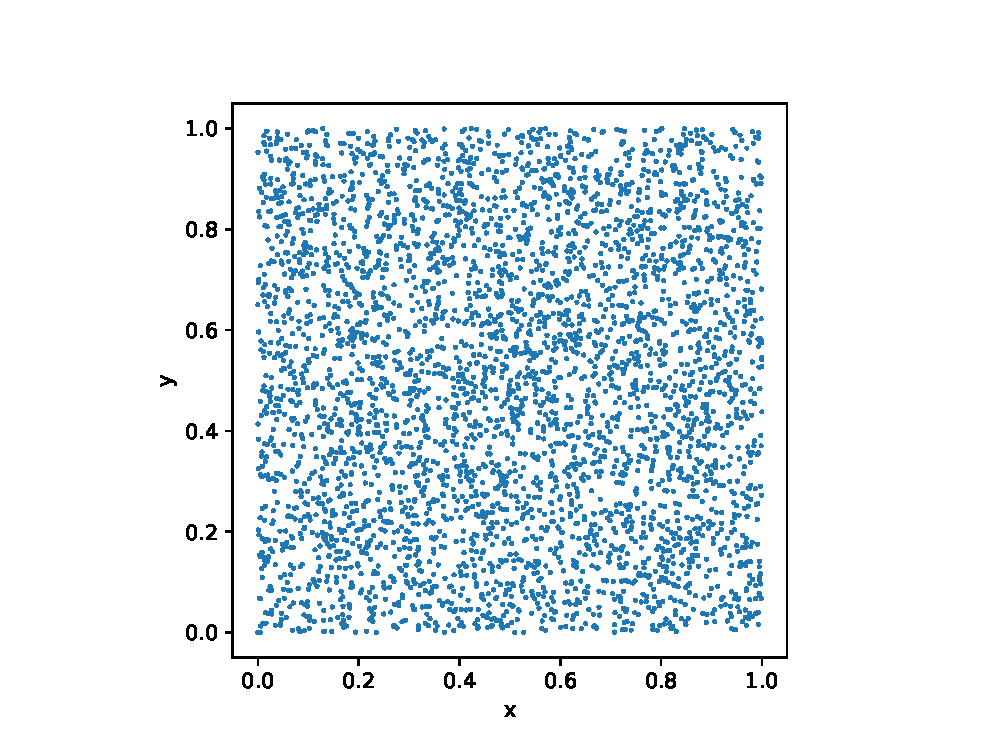
\includegraphics[width=0.48\textwidth]{rand.eps}}
    \hfill
    \subfloat[20000个随机数平面分布图]{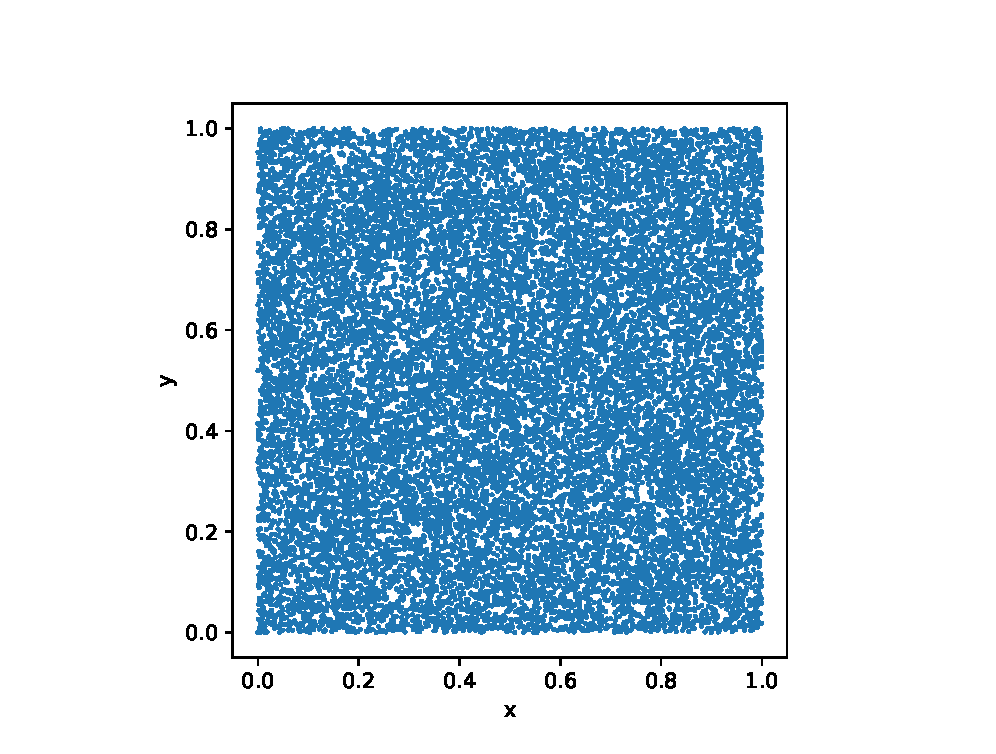
\includegraphics[width=0.48\textwidth]{randd.eps}}
    \hfill
    \subfloat[40000个随机数平面分布图]{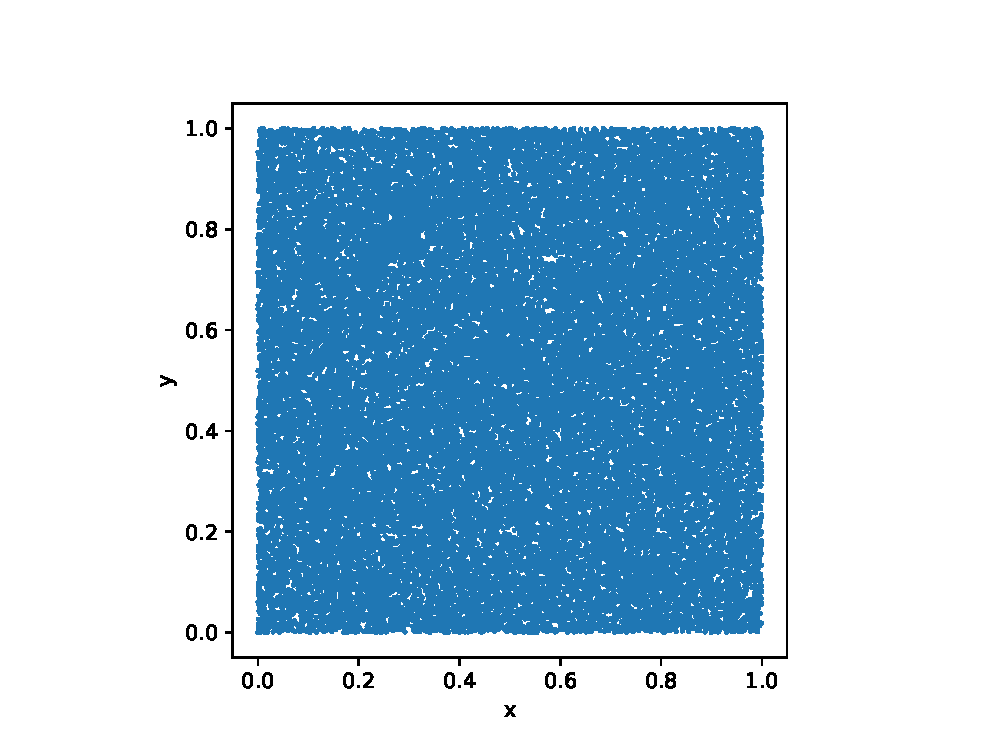
\includegraphics[width=0.48\textwidth]{randdd.eps}}
    \caption{随机数平面分布图}
\end{figure}
\newpage
    \item[(b)] \textbf{k阶矩检验均匀性}\\
        将 \texttt{moments.out}中的数据整理列表如下,保留小数点后四位,将
        $\langle x^k \rangle$与 $1/(k+1)$比较,可以观察出,随着$N$增大,
        $\langle x^k \rangle$的值越来越趋近 $1/(k+1)$.\\
\begin{table*}[h]
\scriptsize
\begin{center}
\begin{tabular}{|l|c|c|c|c|c|c|c|c|c|c|}
    \hline
    \diagbox{$N$}{$\langle x^k \rangle$}{$k$} & 1 & 2 & 3 & 4 & 5 & 6 & 7 & 8 &
    9 & 10\\
    \hline
    $10^2$ & 0.4857 & 0.3245 & 0.2474 &
    0.2028 & 0.1739 & 0.1536 &
    0.1386 & 0.1269 & 0.1176 & 0.1098 \\
    \hline
    $10^3$ & 0.5022 & 0.3312 & 0.2461 & 0.1959 & 0.1628 & 0.1395 & 0.1222 & 0.1087
                  & 0.0981 & 0.0893 \\
    \hline
    $10^4$ & 0.4982 &       0.3318  &     0.2488   &
    0.1990   &    0.1658   &    0.1421
                          & 0.1243   &    0.1105  &
    0.0995 &  0.0904 \\
    \hline
    $10^5$ & 0.4997   &    0.3329   &
    0.2495  &    0.1996   &    0.1664 &
    0.1426   &    0.1248  &    0.1109
                          & 0.0999 & 0.0908 \\ 
    \hline
    $10^6$ & 0.4999   &    0.3332  &
    0.2498   &    0.1998   &    0.1665
                          &0.1427   &    0.1248  &
    0.1109   &     0.0998 &  0.0907 \\
    \hline
    $10^7$ & 0.4999   &    0.3333  &
    0.2499   &    0.1999  &     0.1666  &
    0.1428   &    0.1249  &     0.1110
                          & 0.0999 &  0.0908 \\
    \hline
    $1/(k+1)$ & 0.5000 & 0.3333 & 0.2500 & 0.2000 & 0.1667 & 0.1428 & 0.1250 &
    0.1111 & 0.0100 & 0.0909 \\
    \hline
\end{tabular}
\caption{随机数序列$k$阶矩数值}
\end{center}
\end{table*}
\newline
再将 \texttt{difference.out}中的数据整理列表,表中数据为 $\left | \langle x^k
\rangle-1/(k+1)\right |$的值。观察可得:偏差的数值总是小于
$1/\sqrt{N}$的数值,这表明生成随机数的均匀性优良.\\
\begin{table*}[h]
\tiny
\begin{center}
\begin{tabular}{|l|l|l|l|l|l|l|l|l|l|l|l|}
\hline
\diagbox{$N$}{$k$} &      1       & 2
                                                    &     3       & 4
                                                    &      5      & 6
                                                    &   7         & 8
                                                    &     9       &
10 &                                                    $1/\sqrt{N}$        \\ \hline
 $10^2$ & 1.427e-2 & 8.820e-3 & 2.557e-3 & 2.836e-3 & 7.240e-3 & 1.078e-2 & 1.360e-2 & 1.584e-2 & 1.760e-2 & 1.898e-2 & 1.000e-1\\ \hline
 $10^3$ & 2.281e-3 & 2.114e-3 & 3.823e-3 & 4.095e-3 & 3.788e-3 & 3.296e-3 & 2.783e-3 & 2.311e-3 & 1.898e-3 & 1.544e-3 & 3.162e-2\\ \hline
 $10^4$ & 1.778e-3 & 1.439e-3 & 1.199e-3 & 9.965e-4 & 8.312e-4 & 7.044e-4 & 6.111e-4 & 5.437e-4 & 4.949e-4 & 4.589e-4 & 1.000e-2\\ \hline
 $10^5$ & 2.840e-4 & 4.224e-4 & 4.013e-4 & 3.305e-4 & 2.561e-4 & 1.941e-4 & 1.474e-4 & 1.146e-4 & 9.270e-5 & 7.868e-5 & 3.162e-3\\ \hline
 $10^6$ & 2.948e-5 & 1.151e-4 & 1.442e-4 & 1.488e-4 & 1.453e-4 & 1.400e-4 &
 1.348e-4 & 1.301e-4 & 1.260e-4 & 1.224e-4 & 1.000e-3\\ \hline
 $10^7$ & 1.856e-5 & 3.198e-5 & 3.946e-5 & 4.534e-5 & 5.016e-5 & 5.395e-5 & 5.678e-5 & 5.876e-5 & 6.000e-5 & 6.062e-5 & 3.162e-4\\ \hline
\end{tabular}
\caption{$k$阶矩与$1/(k+1)$偏差数值}
\end{center}
\end{table*}
\newpage
\item [(c)] \textbf{自相关系数检验 2 维独立性}\\
    将输出文件 \texttt{indep.out}中的数据整理如下,可观察出
    $C(l)$的值随着数目$N$增大而逐渐减小,其值基本保持在预估值
    $1/\sqrt{N}$的量级甚至更小,这表明在自相关系数检验下,16807产生器产生的随机数独立性较好.
\begin{table*}[h]
\centering
\begin{tabular}{|l|l|l|l|l|l|l|}
\hline
\diagbox{$l$}{$C(l)$}{$N$}  & $10^2$   & $10^3$   & $10^4$   & $10^5$   & $10^6$   & $10^7$   \\ \hline
1 & 5.914e-2 & 4.035e-2 & 3.132e-7 & 2.426e-3 & 2.709e-4 & 3.444e-4 \\ \hline
2 & 9.297e-2 & 3.047e-2 & 1.175e-2 & 2.705e-3 & 1.720e-3 & 3.892e-5 \\ \hline
3 & 4.510e-2 & 4.889e-3 & 5.929e-3 & 3.452e-3 & 8.768e-4 & 3.613e-4 \\ \hline
4 & 4.958e-3 & 3.291e-2 & 7.180e-5 & 3.826e-3 & 3.790e-4 & 4.476e-5 \\ \hline
$1/\sqrt{N}$ & 1.000e-1 & 3.162e-2 & 3.162e-2 & 3.162e-3 & 1.000e-3 & 3.162e-4
\\ \hline  
\end{tabular}
\caption{自相关系数$C(l)$数值}
\end{table*}
\end{enumerate}
\section{结论}
本作业使用Schrage方法编写了随机数产生器程序,并对产生的随机数进行了均匀性和独立性检验,通过自己的程序实现证明了线性同余法随机数产生器
\textsl{(LCG)}基本性质的优良,并可在日后的其他场合下随时调用。但不存在完美的随机数产生器,
\textsl{LCG}仍存在一定的缺点,在某些情况下仍需要使用更加复杂精巧的随机数产生器。
\end{document}
